\subsection{Design System Build and Integration}
The last step to complete the user story of the SDS is to integrate the system into an application. This chapter explains how to package the SDS and load it into a desired application. It is important that the integration is simple so as not to discourage developers from using the design system. \\

The build process is the first part that is important to understand the integration workflow. Webpack is the build tool used by SDS. As shown in Figure 3 in Chapter 1, the components of the design system are built using Typescript, including the Lit framework and using SCSS for styling. Since Typescript and SCSS are not supported by the browser, they must be processed beforehand. Therefore, Webpack comes into play to compile the code. \\
Webpack uses a configuration file, often called webpack.config.js, to describe the steps by which the code is compiled. This file describes rules that tell Webpack what to do with which files that come into the build pipeline. These rules for SDS look like this:\\
\lstinputlisting[linerange={23-41},firstnumber=23,caption={SDS Webpack rules},label=WebpackRules]{../Code/webpack.config.js}
The rules define regular expressions that are used to assign files with their extensions to the corresponding compilers, which are called loaders in the Webpack world. The loaders used here are build-in. But there are also custom ones that can be integrated into a build process. When using loaders, it is sufficient to include the loader string in the \texttt{use} property of a rule object. For example, in line 25-26, Listing \ref{WebpackRules}, the Typescript loader is matched with the regular expression Typescript to process Typescript files. The same pattern is used in line 34-35, Listing \ref{WebpackRules} to match SCSS files with the default style loader that comes with Webpack.\\
After all the rules for compilation have been set, it is time to define the entry point from which Webpack should start building the project. The \texttt{entry} property in the \texttt{webpack.config.js} file defines the starting point. In the case of SDS, this value is set to \texttt{./src/index.ts}. Since there is only one entry point, this file is responsible for all files needed for SDS. A look at the entry file \ref{IndexSDS} shows that there are several imports of Typescript, but also styling files.
\lstinputlisting[linerange={1-9},firstnumber=1,caption={SDS Webpack rules},label=IndexSDS]{../Code/src/index.ts}
The first 6 lines of the \texttt{index.ts} contains the imports of all components written in the SDS so far. A defined alias in the \texttt{tsconfig.json} and \texttt{webpack.config.js} allows to shorten the import path for components. With the import of the component files, which look similar to the button component presented above, the web components are automatically added as custom elements and can be used. In the future, this import might change, as software might not want to load all components at once. \\
The last three lines from 7-9 represent imports of styles. These could be written into a single large file, but for readability they are separated. Essentially, these files contain defined design tokens for colors, spacing and sizes for components and patterns. As an example, the \texttt{colors.scss} looks like this:
\lstinputlisting[linerange={1-15},firstnumber=1,caption={SDS color design tokens},label=ColorTokens]{../Code/src/atoms/colors.scss}
The styling file consists mainly of defined CSS variables. These variables can be overwritten by any software that loads the design system. By changing the rules, the style changes are applied to all components in the entire design system. To avoid having to go into the source code to find out how the various tokens are called, the documentation provides a page (Figure \ref{sds_color_design_tokens}) for reference.
\begin{figure}[htbp]
    \centerline{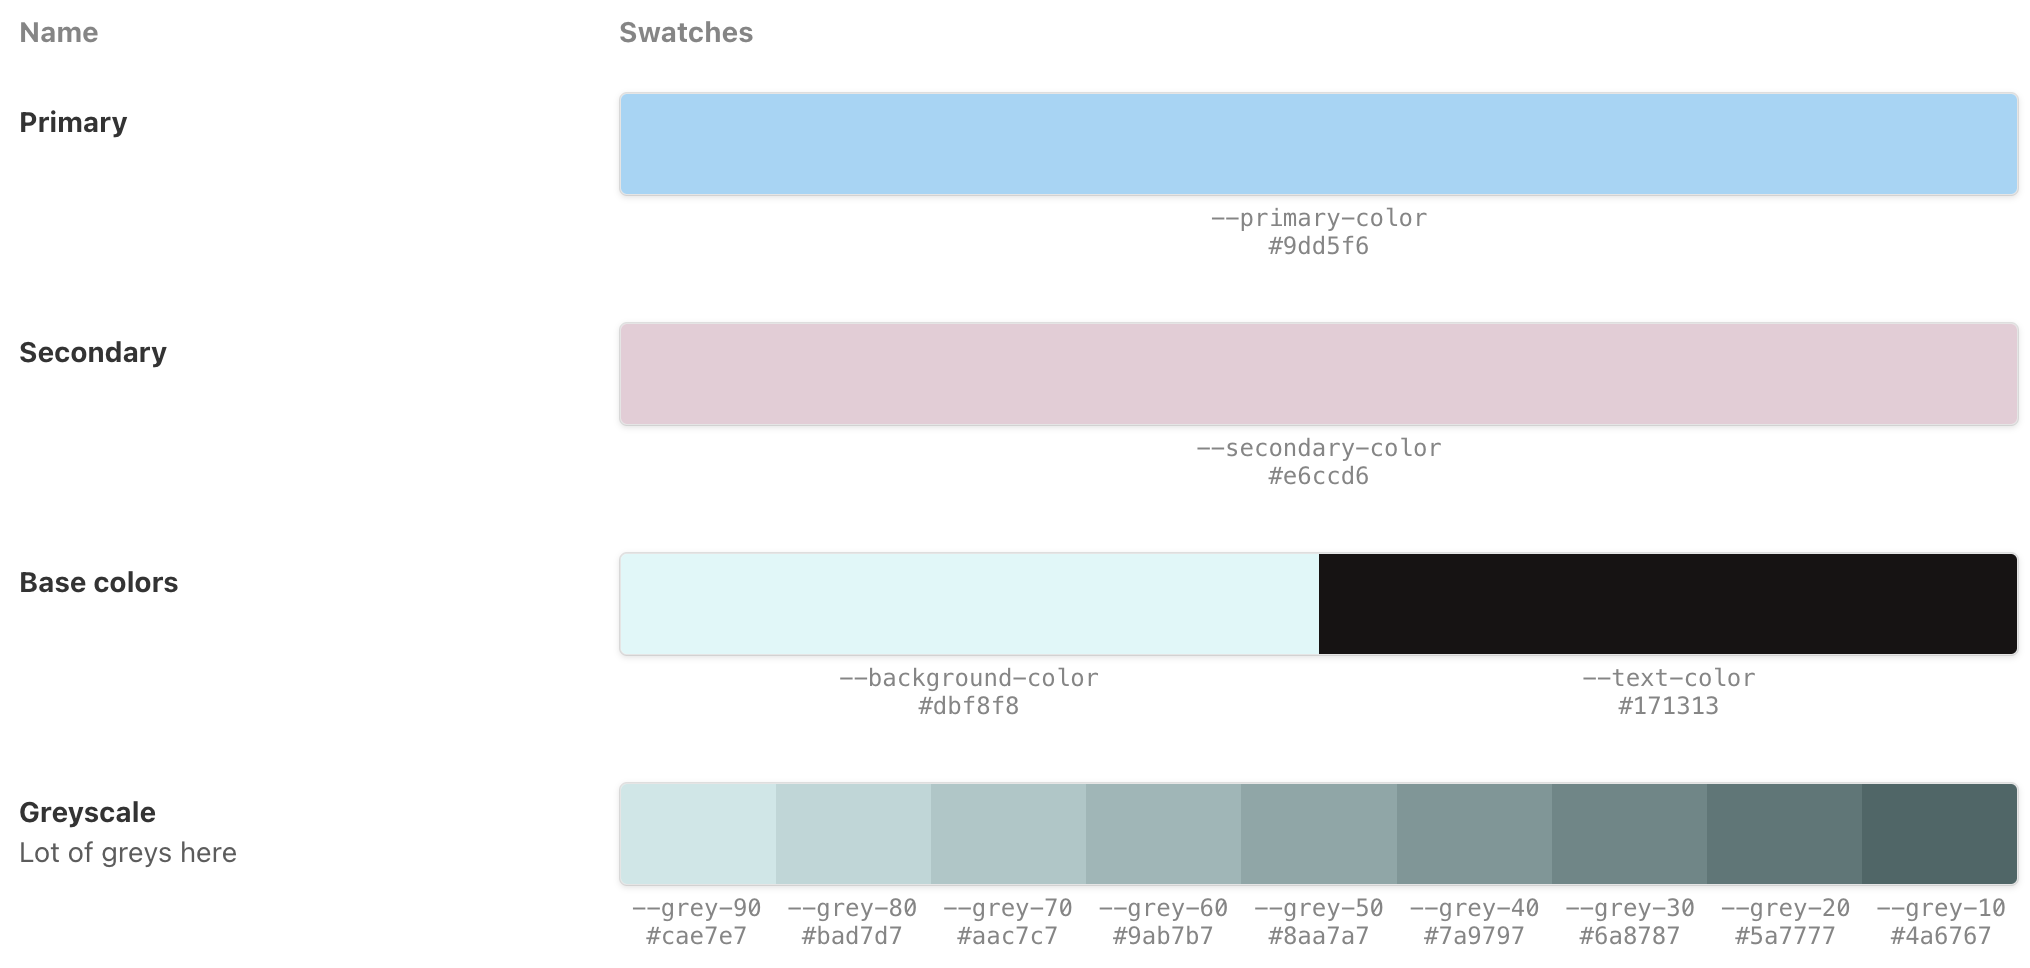
\includegraphics[width=\linewidth]{images/color_design_tokens.png}}
    \caption{SDS color design tokens documentation}
    \label{sds_color_design_tokens}
\end{figure} \\
At a later stage in the design system, the complexity of the styling files may change. For this reason, the SDS uses SCSS to take advantage of its feature of using mixins to create more complex rule sets.\citep{scss_sass_nodate} \\
After all source files have been compiled into browser-readable code, the sources are bundled into two files. One file contains the Javascript code. This code is used to register the custom elements and provide the logic needed in them. The other file, as a result of the build process, is a CSS file that contains all the styles defined in the previously included design token files. For the design system to work properly, both files must be included in a software environment. \\

Last but not least, the bundled files have to be loaded into existing projects. To make them globally available to all, so-called package managers such as NPM are used to publish versions of the software created. In the case of this elaboration, the step to publish the bundled files is omitted. The files are loaded directly from the build folder into the project. The files can either be loaded via \texttt{<script>} and \texttt{<link>} tag within an HTML file or included in the build process of the project. The only requirement is that they are both included. \\
To conclude this chapter on the build of the SDS and how it can be integrated into existing or new projects. The next chapter will look at a project that uses SDS and compare it to a project that does not. The testing of both softwares will shed light on whether such a design system can contribute to the standardisation of user interfaces for SaaS software. 
